% Created by tikzDevice version 0.12.3.1 on 2022-03-12 18:17:51
% !TEX encoding = UTF-8 Unicode
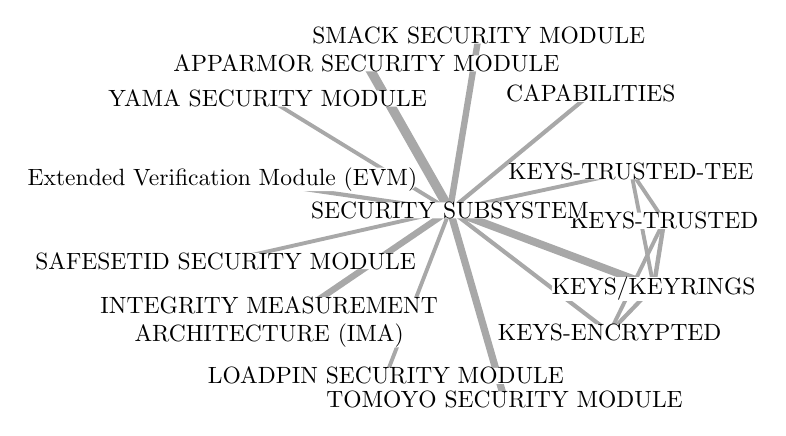
\begin{tikzpicture}[
	x=1pt,y=1pt,
	node/.style={rounded corners,fill=white}
]
\definecolor{fillColor}{RGB}{255,255,255}
%\path[use as bounding box,fill=fillColor,fill opacity=0.00] (0,0) rectangle (375.80,289.08);
\begin{scope}
%\path[clip] (  0.00,  0.00) rectangle (375.80,289.08);
\definecolor{fillColor}{RGB}{255,255,255}

%\path[fill=fillColor] (  0.00,  0.00) rectangle (375.80,289.08);
\end{scope}
\begin{scope}
%\path[clip] ( 32.75, 32.75) rectangle (345.80,259.08);
\definecolor{drawColor}{gray}{0.66}

\path[draw=drawColor,line width= 3.4pt,line join=round] (156.11,200.58) -- (186.30,147.46);

\path[draw=drawColor,line width= 1.5pt,line join=round] (237.21,189.50) -- (186.30,147.46);

\path[draw=drawColor,line width= 1.5pt,line join=round] (104.08,159.42) -- (186.30,147.46);

\path[draw=drawColor,line width= 2.3pt,line join=round] (120.96,102.99) -- (186.30,147.46);

\path[draw=drawColor,line width= 1.4pt,line join=round] (244.03,103.30) -- (263.72,143.69);

\path[draw=drawColor,line width= 1.5pt,line join=round] (244.03,103.30) -- (259.92,119.80);

\path[draw=drawColor,line width= 1.5pt,line join=round] (244.03,103.30) -- (186.30,147.46);

\path[draw=drawColor,line width= 1.4pt,line join=round] (263.72,143.69) -- (251.70,161.55);

\path[draw=drawColor,line width= 1.6pt,line join=round] (263.72,143.69) -- (259.92,119.80);

\path[draw=drawColor,line width= 1.6pt,line join=round] (263.72,143.69) -- (186.30,147.46);

\path[draw=drawColor,line width= 1.4pt,line join=round] (251.70,161.55) -- (259.92,119.80);

\path[draw=drawColor,line width= 1.4pt,line join=round] (251.70,161.55) -- (186.30,147.46);

\path[draw=drawColor,line width= 2.8pt,line join=round] (259.92,119.80) -- (186.30,147.46);

\path[draw=drawColor,line width= 1.4pt,line join=round] (163.14, 87.65) -- (186.30,147.46);

\path[draw=drawColor,line width= 1.4pt,line join=round] (105.23,129.11) -- (186.30,147.46);

\path[draw=drawColor,line width= 2.3pt,line join=round] (186.30,147.46) -- (196.72,210.55);

\path[draw=drawColor,line width= 2.6pt,line join=round] (186.30,147.46) -- (206.02, 79.10);

\path[draw=drawColor,line width= 1.4pt,line join=round] (186.30,147.46) -- (120.41,187.83);
\definecolor{fillColor}{RGB}{255,255,255}


\end{scope}
\begin{scope}
%\path[clip] ( 32.75, 32.75) rectangle (345.80,259.08);
\definecolor{drawColor}{RGB}{0,0,0}

\node[node,text=drawColor,anchor=base,inner sep=0pt, outer sep=0pt, scale=  0.85] at (156.11,197.64) {APPARMOR SECURITY MODULE}; % (156.11,200.64)
\definecolor{fillColor}{RGB}{255,255,255}


\end{scope}
\begin{scope}
%\path[clip] ( 32.75, 32.75) rectangle (345.80,259.08);
\definecolor{drawColor}{RGB}{0,0,0}

\node[node,text=drawColor,anchor=base,inner sep=0pt, outer sep=0pt, scale=  0.85] at (237.21,186.57) {CAPABILITIES}; % (237.21,196.57)
\definecolor{fillColor}{RGB}{255,255,255}


\end{scope}
\begin{scope}
%\path[clip] ( 32.75, 32.75) rectangle (345.80,259.08);
\definecolor{drawColor}{RGB}{0,0,0}

\node[node,text=drawColor,anchor=base,inner sep=0pt, outer sep=0pt, scale=  0.85] at (104.08,156.49) {Extended Verification Module (EVM)};
\definecolor{fillColor}{RGB}{255,255,255}


\end{scope}
\begin{scope}
%\path[clip] ( 32.75, 32.75) rectangle (345.80,259.08);
\definecolor{drawColor}{RGB}{0,0,0}

\node[node,text=drawColor,anchor=base,inner sep=0pt, outer sep=0pt, scale=  0.85, align=center] at (120.96,100.05) {INTEGRITY MEASUREMENT\\ARCHITECTURE (IMA)};
\definecolor{fillColor}{RGB}{255,255,255}


\end{scope}
\begin{scope}
%\path[clip] ( 32.75, 32.75) rectangle (345.80,259.08);
\definecolor{drawColor}{RGB}{0,0,0}

\node[node,text=drawColor,anchor=base,inner sep=0pt, outer sep=0pt, scale=  0.85] at (244.03,100.36) {KEYS-ENCRYPTED};
\definecolor{fillColor}{RGB}{255,255,255}


\end{scope}
\begin{scope}
%\path[clip] ( 32.75, 32.75) rectangle (345.80,259.08);
\definecolor{drawColor}{RGB}{0,0,0}

\node[node,text=drawColor,anchor=base,inner sep=0pt, outer sep=0pt, scale=  0.85] at (263.72,140.75) {KEYS-TRUSTED}; % (263.72,140.75)
\definecolor{fillColor}{RGB}{255,255,255}


\end{scope}
\begin{scope}
%\path[clip] ( 32.75, 32.75) rectangle (345.80,259.08);
\definecolor{drawColor}{RGB}{0,0,0}

\node[node,text=drawColor,anchor=base,inner sep=0pt, outer sep=0pt, scale=  0.85] at (251.70,158.61) {KEYS-TRUSTED-TEE}; % (271.70,168.61)
\definecolor{fillColor}{RGB}{255,255,255}


\end{scope}
\begin{scope}
%\path[clip] ( 32.75, 32.75) rectangle (345.80,259.08);
\definecolor{drawColor}{RGB}{0,0,0}

\node[node,text=drawColor,anchor=base,inner sep=0pt, outer sep=0pt, scale=  0.85] at (259.92,116.86) {KEYS/KEYRINGS}; % (279.92,126.86)
\definecolor{fillColor}{RGB}{255,255,255}


\end{scope}
\begin{scope}
%\path[clip] ( 32.75, 32.75) rectangle (345.80,259.08);
\definecolor{drawColor}{RGB}{0,0,0}

\node[node,text=drawColor,anchor=base,inner sep=0pt, outer sep=0pt, scale=  0.85] at (163.14, 84.71) {LOADPIN SECURITY MODULE};
\definecolor{fillColor}{RGB}{255,255,255}


\end{scope}
\begin{scope}
%\path[clip] ( 32.75, 32.75) rectangle (345.80,259.08);
\definecolor{drawColor}{RGB}{0,0,0}

\node[node,text=drawColor,anchor=base,inner sep=0pt, outer sep=0pt, scale=  0.85] at (105.23,126.17) {SAFESETID SECURITY MODULE};
\definecolor{fillColor}{RGB}{255,255,255}


\end{scope}
\begin{scope}
%\path[clip] ( 32.75, 32.75) rectangle (345.80,259.08);
\definecolor{drawColor}{RGB}{0,0,0}

\node[node,text=drawColor,anchor=base,inner sep=0pt, outer sep=0pt, scale=  0.85] at (186.30,144.52) {SECURITY SUBSYSTEM};
\definecolor{fillColor}{RGB}{255,255,255}


\end{scope}
\begin{scope}
%\path[clip] ( 32.75, 32.75) rectangle (345.80,259.08);
\definecolor{drawColor}{RGB}{0,0,0}

\node[node,text=drawColor,anchor=base,inner sep=0pt, outer sep=0pt, scale=  0.85] at (196.72,207.61) {SMACK SECURITY MODULE};
\definecolor{fillColor}{RGB}{255,255,255}


\end{scope}
\begin{scope}
%\path[clip] ( 32.75, 32.75) rectangle (345.80,259.08);
\definecolor{drawColor}{RGB}{0,0,0}

\node[node,text=drawColor,anchor=base,inner sep=0pt, outer sep=0pt, scale=  0.85] at (206.02, 76.16) {TOMOYO SECURITY MODULE}; % (206.02, 81.16)
\definecolor{fillColor}{RGB}{255,255,255}


\end{scope}
\begin{scope}
%\path[clip] ( 32.75, 32.75) rectangle (345.80,259.08);
\definecolor{drawColor}{RGB}{0,0,0}

\node[node,text=drawColor,anchor=base,inner sep=0pt, outer sep=0pt, scale=  0.85] at (120.41,184.89) {YAMA SECURITY MODULE};
\end{scope}
\end{tikzpicture}

